\documentclass[10pt,t]{beamer}
\usetheme{Heverlee}

%\usepackage[orientation=landscape,size=custom,width=16,height=9,scale=0.45,debug]{beamerposter}

\usepackage{svg}
\usepackage{adjustbox}
\usepackage{amsmath,amssymb}
\usepackage{bm}
\usepackage{tikz} % serve per fare i grafici
\usetikzlibrary{shapes,quotes,arrows.meta}
\usepackage{xcolor}
\usepackage{subcaption}
\usepackage{graphicx}
\usepackage{tabularx}
\usepackage{siunitx}
\usepackage{colortbl}

\usepackage{stanli}


%%% QUICK OPTIONS:
% (A) Math font without serifs, enable line below to make math serif:
    %\usefonttheme[onlymath]{serif}

% (B) Re-define primary colour by adjusting the RGB values
    %\definecolor{pblue}	{RGB}{206,125,66}

% (C) Title page graphic (optional) --- this is not for the background image, see \usebackgroundtemplate to change that ---
    %\titlegraphic{\includegraphics[height=2.7cm]{example_figure.pdf}}

% (D) Add logo to bottom right-corner (optional)
    \logo{\includegraphics[height=0.82cm]{images/logo-polimi.png}\hspace{8pt}\vspace{-6pt}}      

% (E) Choose one (or none) of these lines to add footline bar on all frames
    %\setbeamertemplate{footline}[infoline]  % author, title, insitute
    %\setbeamertemplate{footline}[navigation] % dots swhowing progress
    %\setbeamertemplate{footline}[navsym] % navigation symbols

% (F) Widescreen 16:9 ratio
    %\usepackage[orientation=landscape,size=custom,width=16,height=9,scale=0.45,debug]{beamerposter} 


\setbeamertemplate{footline}[navigation]
\setbeamertemplate{caption}[numbered]

%%% TITLE PAGE INFO:
\title[Heverlee \LaTeX\ Beamer theme]{Coupling multi-body and fluid dynamics analysis}
\subtitle{with preCICE and MBDyn}
\author{Claudio Caccia \and Pierangelo Masarati}
\institute{Politecnico di Milano}
\date{June 2021}

% Text inside {} is used on the title page. Text inside [] is optional, and is used in footline bar (if [] is omitted then text from {} will be used in both ; if [] is specified but left empty then the footline will not show any text)



\makeatletter
\let\beamer@writeslidentry@miniframeson=\beamer@writeslidentry%
\def\beamer@writeslidentry@miniframesoff{%
  \expandafter\beamer@ifempty\expandafter{\beamer@framestartpage}{}% does not happen normally
  {%else
    % removed \addtocontents commands
    \clearpage\beamer@notesactions%
  }
}
\newcommand*{\miniframeson}{\let\beamer@writeslidentry=\beamer@writeslidentry@miniframeson}
\newcommand*{\miniframesoff}{\let\beamer@writeslidentry=\beamer@writeslidentry@miniframesoff}
\makeatother




 %%
 %%  0. TITLE PAGE and TABLE OF CONTENT
 %%
\begin{document}
% Title page

% Change image, or delete this line to remove background image
% TODO get image

%{\usebackgroundtemplate{ \parbox[b][\paperheight][b]{\paperwidth}{\centering\includegraphics[width=\paperwidth]{Background/bg_alishan.jpg}}} 
 %   abudhabi      cherry      forest      river
 %   alishan       chobe       leuven      sanfancisco
 %   blueprint     columns     library     uyuni
 %   bokeh         flowers     newyork     winter

%\setbeamercolor{background canvas}{bg=lgray}  % make background light gray

%\begin{frame}[plain,noframenumbering]
%    \titlepage
%\end{frame}
%}		

{\usebackgroundtemplate{ \parbox[b][\paperheight][b]{\paperwidth}{\centering\includegraphics[width=\paperwidth]{Personal_BG/ry06mg.jpg}}} 

\begin{frame}[plain,noframenumbering]
    \titlepage
\end{frame}
}


% Table of contents slide
\begin{frame}{Outline}
	%\vskip 2mm
	%text?
	%\vskip 2mm
	\hfill	{\parbox{.95\textwidth}{\tableofcontents[hideothersubsections]}}
\end{frame}


% SECTION 1
%\section[FSI techniques]{FSI solution techniques}









\section{MBDyn features}

\begin{frame}{\includegraphics[width=.18\textwidth]{images/mbdyn.png} }

\textbf{\textcolor{dorange}{M}ulti\textcolor{dorange}{B}ody \textcolor{red}{DYN}amics analysis} software (\url{www.mbdyn.org}).\\


\vspace{5mm}

Main features:

    \begin{itemize}
        \item simulation of linear and non-linear \textbf{\textcolor{dorange}{dynamics}}
        \item definition of rigid and flexible elements:\\ \textbf{\textcolor{dblue}{beams}}, shells, component mode synthesis elements...
        \item subject to \textbf{\textcolor{pblue}{kinematic constraints}} and \textbf{\textcolor{indigo}{external forces}}
        \item possibly governed by \textbf{\textcolor{fgreen}{control subsystems}}
    \end{itemize}

\pause
\vspace{5mm}

Open to perform multi-physics simulations:
\begin{itemize}
    \item \textcolor{teal}{\textbf{steer}} the simulation
    \item \textcolor{teal}{\textbf{map}} between \textit{nodes} and external points:
    \begin{itemize}
    \footnotesize
        \item \textcolor{fgreen}{\textbf{pass}} externally computed forces to MBDyn
        \item \textcolor{indigo}{\textbf{retrieve}} point displacements
    \end{itemize}
\end{itemize}

\end{frame}


\begin{frame}{External Structural Mapping}

\textcolor{teal}{\textbf{Decoupling geometry and structural properties}:} 

\begin{figure}
  \begin{subfigure}[t]{.486\textwidth}
    \centering
    \includegraphics[width=\linewidth]{images/beams_1a.png}
    \caption{Model: \textbf{nodes} and \textbf{beams}}
  \end{subfigure}
  \hfill
  \begin{subfigure}[t]{.486\textwidth}
    \centering
    \includegraphics[width=\linewidth]{images/interf_1a.png}
    \caption{interface geometry: \textbf{shape}}
  \end{subfigure}

  \bigskip

  \begin{subfigure}[t]{.486\textwidth}
    \centering
    \includegraphics[width=\linewidth]{images/mesh_1b.png}
    \caption{interface mesh: \textbf{MLS mapping}}
  \end{subfigure}
  \hfill
  \begin{subfigure}[t]{.486\textwidth}
    \centering
    \includegraphics[width=\linewidth]{images/whole_1aa.png}
    \caption{\textbf{coupling} to CFD solver}
  \end{subfigure}
\end{figure}


\end{frame}



\begin{frame}{FSI Simulations using MBDyn}

\begin{figure}
    \centering
    \begin{tikzpicture}
        \node[inner sep=0pt] (mbdyn) at (0,0)
            {\includegraphics[width=.25\textwidth]{images/mbdyn.png}};
        \node[inner sep=0pt] (precice) at (0,-2.5)
            {\includegraphics[width=.25\textwidth]{images/precice.png}};
        \node[inner sep=0pt] (of) at (-4,-5) 
            {\includegraphics[width=.2\textwidth]{images/of.jpeg}};
        \node[inner sep=0pt] (su2) at (-1.25,-5) 
            {\includegraphics[width=.12\textwidth]{images/logoSU2.png}};
        \node[inner sep=0pt] (cfd) at (0.5,-5) 
            {\includegraphics[width=.14\textwidth]{images/simulation-CFD.png}};
        \node[inner sep=0pt] (aster) at (4,-5) 
            {\includegraphics[width=.125\textwidth]{images/Logo_aster.png}};
        \draw[<->,thick] (mbdyn.south) -- (precice.north)
            node[midway,fill=white,text=orange] {\large{\textbf{adapter}}};
         \draw[->,thick] (precice.south) -- (of.north east)
            node[midway] {};
         \draw[->,thick] (precice.south) -- (su2.north)
            node[midway,fill=white, text=cyan] {\large{\textbf{FSI}}};
         \draw[->,thick] (precice.south) -- (cfd.north)
            node[midway] {};
         \draw[->,thick] (precice.south) -- (aster.north west)
            node[midway,fill=white, text=teal] {\large{\textbf{SSI}}};
            
\end{tikzpicture}
\end{figure}

\end{frame}






\section{Adapter}

\begin{frame}{MBDyn adapter}

\begin{figure}
    \centering
    \begin{tikzpicture}[scale=0.75]

%MBDyn shape
\draw[black, thick,fill=yellow!10] (0,0) -- (2,0) -- (2,0.5) -- (2.5,0.5) -- (2.5,1.5) -- (2,1.5) -- (2,2) -- (0,2) -- cycle;

%MBDyn logo
\node (mbdyn) at (1.23,1.05) {\includegraphics[width=.14\textwidth]{images/mbdyn.png}};

% left arrow
\draw[<->] (2.5,1.0)-- (5.5,1.0) node[midway,above] {\footnotesize{\texttt{mbcnodal.h}}} node[midway,below] {\footnotesize{\texttt{libmbc.so}}};

% adapter shape
\draw[black, thick, fill={rgb:red,1;green,2;blue,3}] (5.0,0) -- (7.0,0) -- (7.0,0.5) -- (6.5,0.5) -- (6.5,1.5) -- (7.0,1.5) -- (7.0,2.0) -- (5.0,2.0) -- (5.0,1.5) -- (5.5,1.5) -- (5.5,0.5) -- (5.0,0.5) -- cycle;

%adapter text
\node (ad1) at (6.0,1.75) {\textcolor{white}{\footnotesize{\textbf{MBDyn}}}};
\node (ad1) at (6.0,0.25) {\textcolor{white}{\footnotesize{\textbf{adapter}}}};

% right arrow
\draw[<->] (6.5,1.0)-- (9.5,1.0) node[midway,above] {\footnotesize{\texttt{precice.h}}} node[midway,below] {\footnotesize{\texttt{libprecice.so}}};

%precice shape
\draw[black, thick,fill=green!5] (10,0) -- (12,0) -- (12,2.0) -- (10,2.0) -- (10,1.5) -- (9.5,1.5) -- (9.5,0.5) -- (10,0.5) -- cycle;

%precice logo
\node (pc) at (10.75,1.00) {\includegraphics[width=.14\textwidth]{images/preCICE_logo_42px.png}};

%coupling
\draw[<->] (12.0,1.0)-- (14,1.0) node[midway,above] {\footnotesize{\textbf{FSI}}} node[midway,below] {\footnotesize{\textit{coupling}}};

    \end{tikzpicture}
    \caption{MBDyn adapter interface scheme}
    \label{fig:adapter_scheme}
\end{figure}




%    \begin{figure}
%        \centering
%        \includegraphics[width=0.8\textwidth]{images/adapter_scheme.png}
%    \end{figure}
    
    %\vspace{1mm}
    
    \begin{itemize}
     \itemsep 8pt
        \item \textcolor{teal}{\textbf{independent}} from MBDyn code
        \item \textcolor{dblue}{\textbf{APIs}} from preCICE and MBDyn:
        \begin{enumerate}
            \itemsep 5pt
            \item \texttt{libprecice.so}   \hspace{0.6cm} (from preCICE)
            \item \texttt{libmbc.so}       \hspace{1.27cm}    (from MBDyn)
        \end{enumerate}
        
        \item composed of 2 C++ \textcolor{indigo}{\textbf{classes}}:
        \begin{enumerate}
            \itemsep 5pt
            \item perform co-simulation
            \item access and steer the MBDyn simulation, save data
        \end{enumerate}
        
    \end{itemize}
\end{frame}

\begin{frame}{Adapter Input}
  \vspace{1.0cm}
  \begin{description}[Simulation]
  \itemsep 10pt
  \item[preCICE] \textcolor{dorange}{config file, participant name, ...}
  \item[MBDyn]      \textcolor{red}{simulation file} \\
                    \textcolor{red}{socket}: send forces and retrieve displacements \\
  \item[Simulation] \textcolor{teal}{mesh location}: used for coupling and mapping\\
                    \textcolor{teal}{data to pass}: displacements or deltas\\
                    \textcolor{teal}{starting ramp configuration}: type, period, ...
%  \item[Output]     \textcolor{indigo}{vtk file}: location, name, time interval, ...\\
%                    \textcolor{indigo}{resultants}: name, origin for moments, ...
  \end{description}

%    \begin{figure}
%        \centering
%        \includegraphics[width=0.5\textwidth, trim=0 45 0 50,clip]{images/coeff_pres.png}
%        \caption{scaling factor at start}
%    \end{figure}

\end{frame}

\begin{frame}{Adapter Output}

\begin{description}[saved data]
    \item[*.vtu files] at each mapped interface point: \\
                    \textcolor{dorange}{Displacements}, \textcolor{red}{Deltas}\\ 
                    \textcolor{dblue}{Velocities}\\
                    \textcolor{teal}{Forces}
    \item[csv file] with resultants and moments at each $\Delta t$
    \item[MDByn] simulation output parsed through \texttt{python} script
\end{description}



\begin{figure}
 \begin{subfigure}[t]{.486\textwidth}
    \centering
    \includegraphics[width=\linewidth, trim=20 0 0 200,clip]{images/fsi2_disp.png}
    \caption{2D FSI example}
  \end{subfigure}
  \hfill
  \begin{subfigure}[t]{.486\textwidth}
    \centering
    \includegraphics[width=\linewidth]{images/naca_force.png}
    \caption{3D FSI example}
  \end{subfigure}
\end{figure}


\end{frame}

\begin{frame}{Coupling sequence}
    
%Tell something about coupling sequence. 


\begin{columns}


\begin{column}{0.5\textwidth}
\textcolor{dorange}{\textbf{MBDyn}}:

\vspace{0.2cm}

\begin{itemize}
    \item \textcolor{teal}{\textbf{computes}} motion step at $t_k, i_j$
    \item \textcolor{fgreen}{\textbf{sends}} motion to peer
    \item \textcolor{dblue}{\textbf{receives}} forces based on kinematics at $i_j$
    \item \textcolor{indigo}{\textbf{iterates}} until peer converges
\end{itemize}

%\centering
$$f\left(y_k^{(j)},\dot{y}_k^{(j)},u_k^{(j-1)}\right)=0$$

\pause

\begin{itemize}
    \item \textcolor{dorange}{\textbf{MBDyn}} must start first
    \item \textbf{added mass instability} when:
\end{itemize}

$$M = \frac{\rho_f}{\rho_s} > 0.25$$


\end{column}

\pause

\begin{column}{0.5\textwidth}
\textcolor{pblue}{\textbf{preCICE}} adapter:

\vspace{0.2cm}

\begin{itemize}
    \item \textcolor{dblue}{\textbf{retrieves}} data from peer
    \item \textcolor{teal}{\textbf{performs}} computation step
    \item \textcolor{fgreen}{\textbf{sends}} data to peer
    \item \textcolor{indigo}{\textbf{advances}} (acceleration)
\end{itemize}

\pause

\vspace{0.5cm}

\begin{itemize}
    \item update in adapter
    \item one redundant computation, but still outperforms other solutions
    \item might be implemented in MBDyn
\end{itemize}


\end{column}


\end{columns}

    
\end{frame}



\section{Turek Hron Benchmark}





\begin{frame}{Turek-Hron  Benchmark (turek et. al 2006): domain}


\begin{columns}
    \column{0.6\textwidth}
    \begin{figure}[t]
    \vspace*{-1.5cm}
    \hspace*{-0.2cm}
	\centering
	  \begin{subfigure}[t]{\textwidth}
    \centering
    \includegraphics[width=0.865\textwidth, trim=0 0 50 0, clip]{images/FSI2/FSI2.png}
  \end{subfigure}
  \begin{subfigure}[t]{\textwidth}
    %\centering
    \hspace{3pt}
    \includegraphics[width=0.89\textwidth]{images/FSI2/FSI2-mesh.png}
  \end{subfigure}
	
	
	
	
    \end{figure}
    
    \column{0.4\textwidth}
    	\scriptsize
		\begin{tabular}{ c | r } 
			symbol & value [m]  \\
			\hline
			H  & $0.41$     \\
			L  & $2.5$  \\
			l  & $0.35$  \\
			h  & $0.02$  \\
			C  & $\left(0.2,0.2 \right)$  \\
			r  & $0.05$  \\
			\end{tabular}

		\vspace{0.5cm}
		\begin{tabular}{ l c  | c } 
			\multicolumn{2}{c|}{parameter} & value  \\ 
			\hline
			$\rho_F$ & \si{kg.m^{-3}} & \cellcolor{blue!20} $1000$   \\
			$\nu$& \si{m^2.s^{-1}} & \cellcolor{blue!20} $1 \cdot 10^{-3}$  \\
			Re &  & \cellcolor{blue!20} $20 \rightarrow 200$  \\
		%	$\vec{u}_{max}$ & \si{m.s^{-1}} & \cellcolor{blue!20} $1.5$ \\
			$\bar{u}$ & \si{m.s^{-1}} & \cellcolor{blue!20} $0.2 \rightarrow 2 $ \\
			flow & & \cellcolor{blue!20} laminar \\
			\hline
			$\rho_S$ & \si{kg.m^{-3}} & \cellcolor{orange!50} $10^{3} \rightarrow 10^{4}$    \\
			E & \si{MPa} & \cellcolor{orange!50} $1.4 \rightarrow 5.6$    \\
			\hline
			$M$ & & $ \cellcolor{green!10} 0.1 \rightarrow 1$     \\
		%	\hline
		%	$U_R$ & & $ 8.45\cdot 10^{-2}$  \\
		%	$C_Y$ & & $  7.14 \cdot 10^{-4}$  \\			

		\end{tabular}
\end{columns}

\end{frame}

\begin{frame}{Turek-Hron benchmark: tests}
    
    \begin{itemize}
        \item Static and dynamic analysis of the structural part (CSM)
        \item Fixed fluid domain analysis at different velocity (CFD)
        \item Flexible beam analysis in fluid flow (FSI)
    \end{itemize}
    
    we followed the same steps to validate the framework
    
\end{frame}


\section{CSM Test Cases}

\begin{frame}{Structural model}

  \vspace{0.5cm}
  \begin{description}[structural elements]
  \itemsep 10pt

  \item[structural elements] \textcolor{dorange}{\texttt{beams}} connected to 3 \textcolor{dorange}{\texttt{structural nodes}} each \\ ($EA$, $GA$, $EJ$,$GJ_p$)\\
  \item[inertial elements] \textcolor{dorange}{\texttt{bodies}} (i.e. chunks of cantilever) connected to beam nodes ($m$,$I_{ij}$,offset)\\
  \end{description}    


\begin{figure}[htbp!]
    \begin{subfigure}[t]{.486\textwidth}
	    \centering
	    \resizebox{.9\textwidth}{!}{
        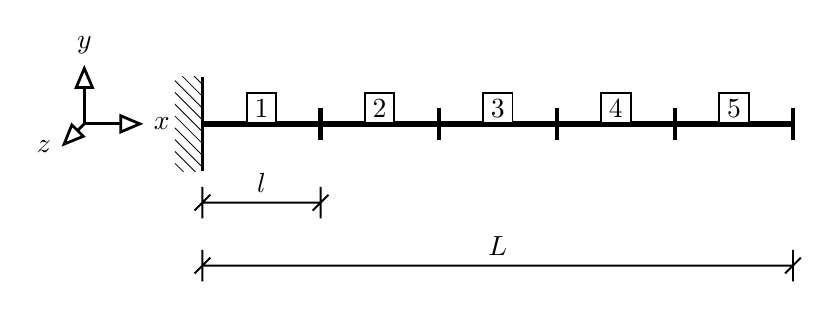
\begin{tikzpicture}
            \point{a}{0}{0};
            \point{b}{1.5}{0};
            \point{c}{3}{0};
            \point{d}{4.5}{0};
            \point{e}{6}{0};
            \point{f}{7.5}{0};
            
            \beam{4}{a}{b};
            \beam{4}{b}{c};
            \beam{4}{c}{d};
            \beam{4}{d}{e};
            \beam{4}{e}{f};
            
            \notation{2}{b}{};
            \notation{2}{c}{};
            \notation{2}{d}{};
            \notation{2}{e}{};
            \notation{2}{f}{};
            
            \notation{4}{a}{b}[ $1$ ];
            \notation{4}{b}{c}[ $2$ ];
            \notation{4}{c}{d}[ $3$ ];
            \notation{4}{d}{e}[ $4$ ];
            \notation{4}{e}{f}[ $5$ ];
            
            \support{3}{a}[-90];
            % \load{1}{b}[90][1][.1];
            
            \dimensioning{1}{a}{f}{-1.8}[$L$];
            \dimensioning{1}{a}{b}{-1}[$l$];
            
            \dscaling{3}{0.5};
            \daxis{1}{-1.5 ,0 ,0}[right][above][left];
        \end{tikzpicture}
        }
    	\caption{Cantilever made of 5 \texttt{beam} elements}
		\label{fig:cnt-beams}
		\end{subfigure}
        \hfill
  \begin{subfigure}[t]{.486\textwidth}
  	    \centering
  	    \resizebox{.9\textwidth}{!}{
        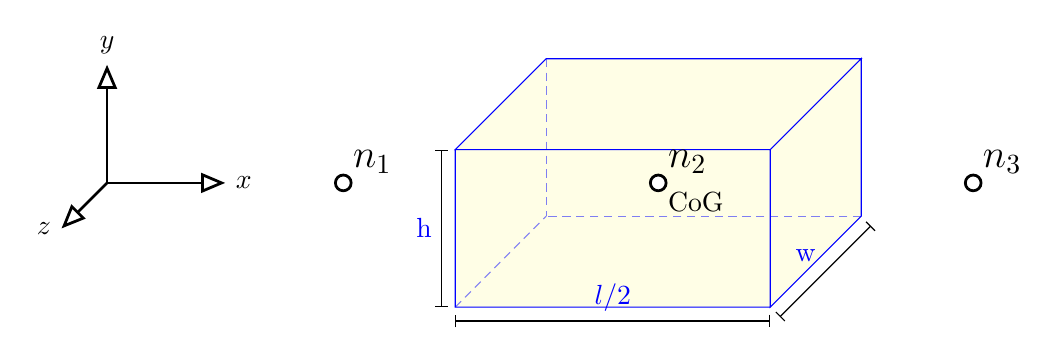
\begin{tikzpicture}[every edge quotes/.append style={auto, text=blue}]
            \pgfmathsetmacro{\cubex}{4}
            \pgfmathsetmacro{\cubey}{2}
            \pgfmathsetmacro{\cubez}{3}
            \draw [draw=blue, every edge/.append style={draw=blue, densely dashed, opacity=.5}, fill=yellow!10]
            (0,0,0) coordinate (o) -- ++(-\cubex,0,0) coordinate (a) -- ++(0,-\cubey,0) coordinate (b) edge coordinate [pos=1] (g) ++(0,0,-\cubez)  -- ++(\cubex,0,0) coordinate (c) -- cycle
            (o) -- ++(0,0,-\cubez) coordinate (d) -- ++(0,-\cubey,0) coordinate (e) edge (g) -- (c) -- cycle
            (o) -- (a) -- ++(0,0,-\cubez) coordinate (f) edge (g) -- (d) -- cycle;
            \path [every edge/.append style={draw=black, |-|}]
            (b) +(0,-5pt) coordinate (b1) edge ["$l/2$"] (b1 -| c)
            (b) +(-5pt,0) coordinate (b2) edge ["h"] (b2 |- a)
            (c) +(3.5pt,-3.5pt) coordinate (c2) edge ["w"] ([xshift=3.5pt,yshift=-3.5pt]e)
            ;
            \daxis{1} {-9,-1,-1.5} [right][above][left];
            %\dpoint{q}{-2.5}{-1}{-1.5};
            \dpoint{r}{-2}{-1}{-1.5};
            \dpoint{s}{-6}{-1}{-1.5};
            \dpoint{t}{2}{-1}{-1.5};
            %\beam{4}{q}{r};
            %\dhinge{1}{q};
            \dhinge{1}{r};
            \dhinge{1}{s};
            \dhinge{1}{t};
            \dnotation{1}{r}{CoG}[below right];
            \dnotation{1}{r}{\Large$n_2$};
            \dnotation{1}{s}{\Large$n_1$};
            \dnotation{1}{t}{\Large$n_3$};
            %\ddimensioning{xy}{q}{r}{1.5}[ $l/4$ ];
            %\ddimensioning{xy}{s}{t}{-2.5}[ $l$ ];
        \end{tikzpicture}
        }
    	\caption{\texttt{Body} attached to node 2 of the \texttt{beam}}
		\label{fig:cnt-mass}
		\end{subfigure}
\end{figure}
\end{frame}



\begin{frame}{CSM Results}

\begin{itemize}
    \item gravitational load
    \item \textcolor{teal}{static} (case 1 and 2, different $E$) or \textcolor{red}{dynamic} (case 3) solution
    \item comparison on \textcolor{dblue}{tip displacement} (\textit{x} and \textit{y} direction)
\end{itemize}
    
\pause

\vspace{0.5cm}
    
\begin{table}[h!]
\footnotesize
%\caption{Comparison of tip displacement (in \si{mm})}
\label{tab:csm}
\begin{center}
\begin{tabular}{ c | c c | c c | c c c }
 & \multicolumn{2}{c|}{CSM1} & \multicolumn{2}{c|}{CSM2} & \multicolumn{3}{c}{CSM3} \\
\hline
\# el. & $u_x$ & $u_y$  & $u_x$ & $u_y$ & $u_x$ & $u_y$  & f  [\si{Hz}]\\
\hline
\cellcolor{green!10}\textbf{4} & \cellcolor{green!10}\textbf{-7.28}    &  \cellcolor{green!10}\textbf{-66.69} & \cellcolor{green!10}\textbf{-0.47} & \cellcolor{green!10}\textbf{-17.13} &  \cellcolor{green!10}\textbf{-14.46}$\pm$\textbf{14.46} & \cellcolor{green!10}\textbf{-65.10}$\pm$\textbf{65.82} & \cellcolor{green!10}\textbf{1.125}  \\
\hline
5 & -7.73    &  -68.68 & -0.51 & -17.67 &  -15.29$\pm$15.29 & -66.69$\pm$68.11 & 1.104 \\
\hline
10 & -8.74    &  -72.90 & -0.58 & -18.83 &  -17.57$\pm$17.57 & -70.82$\pm$71.20 & 1.062 \\
\hline
\hline
\textbf{ref.}  &  \textbf{-7.19} & \textbf{-66.10} & \textbf{-0.47} & \textbf{-16.97} & \textbf{-14.31}$\pm$\textbf{14.31} & \textbf{-63.61}$\pm$\textbf{65.16} & \textbf{1.099} \\
\hline
\end{tabular}
\end{center}
\end{table}

\vspace{0.5cm}

\begin{itemize}
    \item data in \si{mm}
    \item \textcolor{teal}{\textbf{4}} or \textcolor{teal}{\textbf{5}} \textcolor{dorange}{\textbf{\texttt{beam}}} elements give best results
\end{itemize}


\end{frame}





\section{CFD Test Cases}


\begin{frame}{CFD model}


  \vspace{0.5cm}
  \begin{description}[fluid properties]
  \itemsep 10pt

  \item[flow regime] \textcolor{dblue}{laminar}  with \textcolor{dorange}{parabolic} inlet profile\\
  \item[fluid properties] \textcolor{dblue}{viscous} and \textcolor{dorange}{incompressible}\\
  \item[fluid domain] \textcolor{dblue}{rigid}, \textcolor{dorange}{hexahedral mesh}
  \end{description}    


\begin{figure}
    \centering
    \includegraphics[width=\linewidth, trim=0 270 0 200, clip]{images/CFD3.png}
    %\caption{Caption}
    \label{fig:my_label}
\end{figure}


\end{frame}

\begin{frame}{CFD Results}

\begin{itemize}
    \item \textcolor{teal}{mean inlet velocity}: $0.2$, $1$, $2$ \si{m.s^{-1}}
    \item comparison on \textcolor{dblue}{forces} on the structure (\textit{lift} and \textit{drag})
    \item we considered different mesh refinements
\end{itemize}
    
\pause

\vspace{0.2cm}

\begin{table}[h!]
\footnotesize
%\caption{Comparison of lift and drag (in \si{N.m^{-1}})}
\label{tab:cfd}
\begin{center}
\begin{tabular}{ c | c c | c c | c c c }
 & \multicolumn{2}{c|}{CFD1} & \multicolumn{2}{c|}{CFD2} & \multicolumn{3}{c}{CFD3} \\
\hline
size & drag & lift  & drag & lift & drag & lift  & f  [\si{Hz}]\\
\hline
25k    & \cellcolor{green!10}14.28 & \cellcolor{green!10}1.11 & 139.49 & 10.77 & 442.53$\pm$4.75 & -17.39$\pm$384.22 & 4.38  \\
\hline
\textbf{49k}    & \cellcolor{green!10}\textbf{14.28}   & \cellcolor{green!10}\textbf{1.11} &
\cellcolor{green!10}\textbf{137.34} & \cellcolor{green!10}\textbf{10.46} &
\cellcolor{green!10}441.45$\pm$5.17 &\cellcolor{green!10} -15.51$\pm$412.03 &\cellcolor{green!10} 4.41 \\
\hline
90k   &         &      &        &       & \cellcolor{green!10} 440.56$\pm$5.44 &\cellcolor{green!10} -14.94$\pm$428.5  &\cellcolor{green!10} 4.43\\ 
\hline
216k    &         &      &        &       & 440.22$\pm$5.68 & -16.35$\pm$431.84 & 4.44 \\
\hline
\hline
\textbf{ref.}  &  \textbf{14.29} & \textbf{1.12} & \textbf{136.7} & \textbf{10.53} & \textbf{439.45}$\pm$\textbf{5.62} & \textbf{-11.89}$\pm$\textbf{437.81} & \textbf{4.3956} \\
\hline
\end{tabular}
\end{center}
\end{table}

\vspace{0.2cm}

\begin{itemize}
    \item data in \si{N.m^{-1}}
    \item at low speed good solutions even with coarse mesh
    \item at higher speed, Lift depends on the mesh size
\end{itemize}


\end{frame}
























\section{FSI Test Cases}



\begin{frame}{Turek-Hron FSI2 Benchmark: simulation}

\begin{columns}

\column{0.5\textwidth}    

\begin{figure}[htb]
\vspace*{-0.8cm}
\centering % <-- added
\begin{subfigure}{0.5\textwidth}
  \includegraphics[width=\linewidth, trim=0 120 0 120, clip]{images/FSI2/fsi2_v1.png}
  \caption{t=5.0s velocity}
  \label{fig:fsi2_v1}
\end{subfigure}\hfil % <-- added
\begin{subfigure}{0.5\textwidth}
  \includegraphics[width=\linewidth, trim=0 120 0 120, clip]{images/FSI2/fsi2_p1.png}
  \caption{t=5.0s pressure}
  \label{fig:fsi2_p1}
\end{subfigure}\hfil % <-- added

\medskip

\begin{subfigure}{0.5\textwidth}
  \includegraphics[width=\linewidth, trim=0 120 0 120, clip]{images/FSI2/fsi2_v2.png}
  \caption{t=5.135s velocity}
  \label{fig:fsi2_v2}
\end{subfigure}\hfil % <-- added
\begin{subfigure}{0.5\textwidth}
  \includegraphics[width=\linewidth, trim=0 120 0 120, clip]{images/FSI2/fsi2_p2.png}
  \caption{t=5.135s pressure}
  \label{fig:fsi2_p2}
\end{subfigure}\hfil % <-- added

\medskip

\begin{subfigure}{0.5\textwidth}
  \includegraphics[width=\linewidth, trim=0 120 0 120, clip]{images/FSI2/fsi2_v3.png}
  \caption{t=5.27s velocity}
  \label{fig:fsi2_v3}
\end{subfigure}\hfil % <-- added
\begin{subfigure}{0.5\textwidth}
  \includegraphics[width=\linewidth, trim=0 120 0 120, clip]{images/FSI2/fsi2_p3.png}
  \caption{t=5.27s pressure}
  \label{fig:fsi2_p3}
\end{subfigure}\hfil % <-- added

%\caption{FSI2: fluid solution}
\label{fig:FSI2_sol}
\end{figure}

\column{0.5\textwidth}

\footnotesize
\begin{itemize}
    \itemsep 10pt
    \item \textbf{MBDyn} model: 10 \texttt{beam3} elements
    \item \textbf{OpenFOAM} model: \texttt{pimpleFOAM}
    \begin{itemize}
        \item $\approx 25k$ \texttt{hex} cells
    \end{itemize}
    \item \textbf{preCICE} configuration:
    \begin{itemize}
        \item serial implicit coupling
        \item mapping: RBF
        \item acceleration: IQN-ILS
    \end{itemize}
    %\pause
    \item \textbf{performance}
    \begin{itemize}
        \item 14.5 avg. iterations to converge
    \end{itemize}
\end{itemize}

\end{columns}

\end{frame}


\begin{frame}{Turek-Hron FSI2 Benchmark: results}

\begin{columns}

\column{0.3\textwidth}
%\vspace{1cm}
comparison made on \\ \textbf{tip displacements}:

\column{0.7\textwidth}


\vspace{-1cm}
\begin{figure}[htbp!]
    %\vspace{-1.8cm}
	%\centering
	\includegraphics[width=0.9\textwidth, trim=20 20 20 20, clip]{images/FSI2/disp_fsi2_pres.png}
\end{figure}


\end{columns}





\footnotesize
\begin{center}
\begin{tabular}{ l | c c | c c  |  } 
	Study & $d_{x\,tip}$ [\si{mm}] & f [\si{Hz}] & $d_{y\,tip}$ [\si{mm}] & f [\si{Hz}] \\ 
	\hline
	\hline
	Benchmark & $-14.58\pm12.44$ & $3.8$ & $1.23\pm80.6$ & $2.0$ \\
	Turek et al. (2010) & $-14.85\pm12.70$ & $3.86$ & $1.30\pm81.7$ & $1.93$ \\
	Gjertsen & $-14.83\pm13.11$ & & $1.24\pm81.6$ & \\
	Degroote & $-14.07\pm12.37$ & $3.7$ & $1.18\pm76.5$ & $1.9$ \\
	\hline
	Present study & $-14.95\pm9.85$ & $3.87$ & $2.78\pm83.39$ & $1.93$ \\ 
\end{tabular}
    
\end{center}
\vspace{0.2cm}
% Axial flexibility of beams?

\end{frame}







\section{Conclusions}

\begin{frame}{Conclusions}

%\large

\textcolor{pblue}{\textbf{Goals}}:

\begin{itemize}
    \item Exploit \textcolor{pblue}{\textbf{MBDyn}} capabilities to perform fluid-structure co-simulation
    \item Integrate \textit{MBDyn} with \textcolor{pblue}{\textbf{preCICE}} to guarantee a common interface to multiple CFD solvers
    \item validate the \textcolor{pblue}{\textbf{FSI}} simulation with the proposed setup
\end{itemize}

\pause

\vspace{0.5cm}

\textcolor{teal}{\textbf{Results}}:

\begin{itemize}
    \item the \textcolor{teal}{\textbf{adapter}} has been developed and verified
    \item Solutions comparable with \textcolor{teal}{\textbf{benchmarks}} (Turek-Hron, bluff body...)
\end{itemize}

\pause

\vspace{0.5cm}

\textcolor{dorange}{\textbf{Open points}}:

\begin{itemize}
    \item Possible improvement in computation and data exchange between MBDyn and preCICE 
\end{itemize}



\end{frame}

\begin{frame}{Future Development}

\textbf{Three} possible directions of further development:

\vspace{0.3cm}

%\pause

\begin{enumerate}
    \item \textcolor{pblue}{\textbf{Software side}}
        \itemsep 10pt
        \begin{itemize}
            \item improve usability
            \item reduce/avoid redundancy
            \item internal optimizations (data handling, mesh topology...)
        \end{itemize}    

%\pause
    
    \item \textcolor{pblue}{\textbf{Simulation side}}
    
        \begin{itemize}
            \item Reduce, possibly solve, convergence issues with \textit{mass ratio}
            \item Verify scalability, with more complex 3D cases
        \end{itemize}

%\pause
    
    \item \textcolor{pblue}{\textbf{Application side}}
    
        \begin{itemize}
            \item Find further, different benchmarks (other than incompressible flow), users and cases
            \item Use or extend this setup also for \textbf{SSI} problems 
        \end{itemize}
    
\end{enumerate}


\end{frame}


\setbeamercolor{background canvas}{bg=pblue}
\begin{frame}[c,plain]{}
    \centering
    \large{\textcolor{white}{\textbf{Thank you}}}
\end{frame}


\miniframesoff
\setbeamercolor{background canvas}{bg=white}













%%%%%%%%%%%%%%%%%%%%%%%%%%%%%%%%%%%%%%%%%%%%%%%%%%%%%%%%%%%%%%%%%%%%%%%%%%%%%%%%%%%%%%%%%5






\end{document}
